\chapter{Appendix Coupling Coefficient}\label{app:coupling}

In this experiment an estimate of the coupling coefficient between a rocket jet and ice is determined. The rocket jet is approximated by a butane lighter. The coupling coefficient is determined by evaluating how much of the energy from the lighter if efficiently going into melting the ice. The experimental setup is seen in figure\ref{fig:coupling}.

\begin{figure}[htb]
\begin{center}
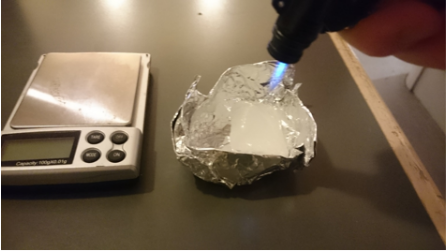
\includegraphics[scale=0.8]{figures/navtheory/coupling}
\caption{Experimental setup}
\label{fig:coupling}
\end{center}
\end{figure}


The lighter is weighed before and after the experiment and it is seen that 0.18 g of butane was used. The energy content in butane is 45.75 MJ/kg, thus the butane used here contained 8235 J. An icecube of 12.64 g was melted. The stating temperature was approximately -23$\circ$ (determined from the temperature of he freezer) and the water puddle ends up being $\sim$20$\circ$. From the specific heat of ice and water the energy it takes to melt and heat it is found. The energy needed for each process for the 12.64 g icecube is seen in figure \ref{fig:lucascouplinggraf} and is 5873 J.
\begin{figure}[htb]
\begin{center}
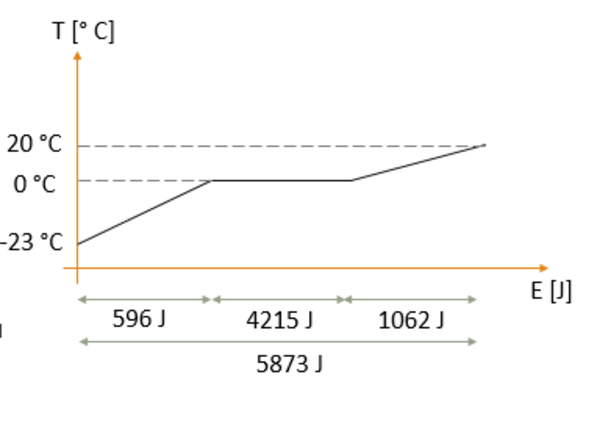
\includegraphics[scale=0.8]{figures/navtheory/couplinggraf}
\caption{Experimental setup}
\label{fig:lucascouplinggraf}
\end{center}
\end{figure}

Thus the coupling coefficient is 

\begin{equation}
\dfrac{5873\ J}{8235 \ J}= 0.71
\end{equation}





% One can also include a script directly like so:
	% \lstinputlisting{path/script.m}